\newpage
\section{Task 2 Robot analysis}
In this section we are going to analyse to KUKA KR6 R900 sixx (Agilus) robot, se figure \ref{fig:KUKA_Agilus}.

\begin{figure}[H]
    \centering
    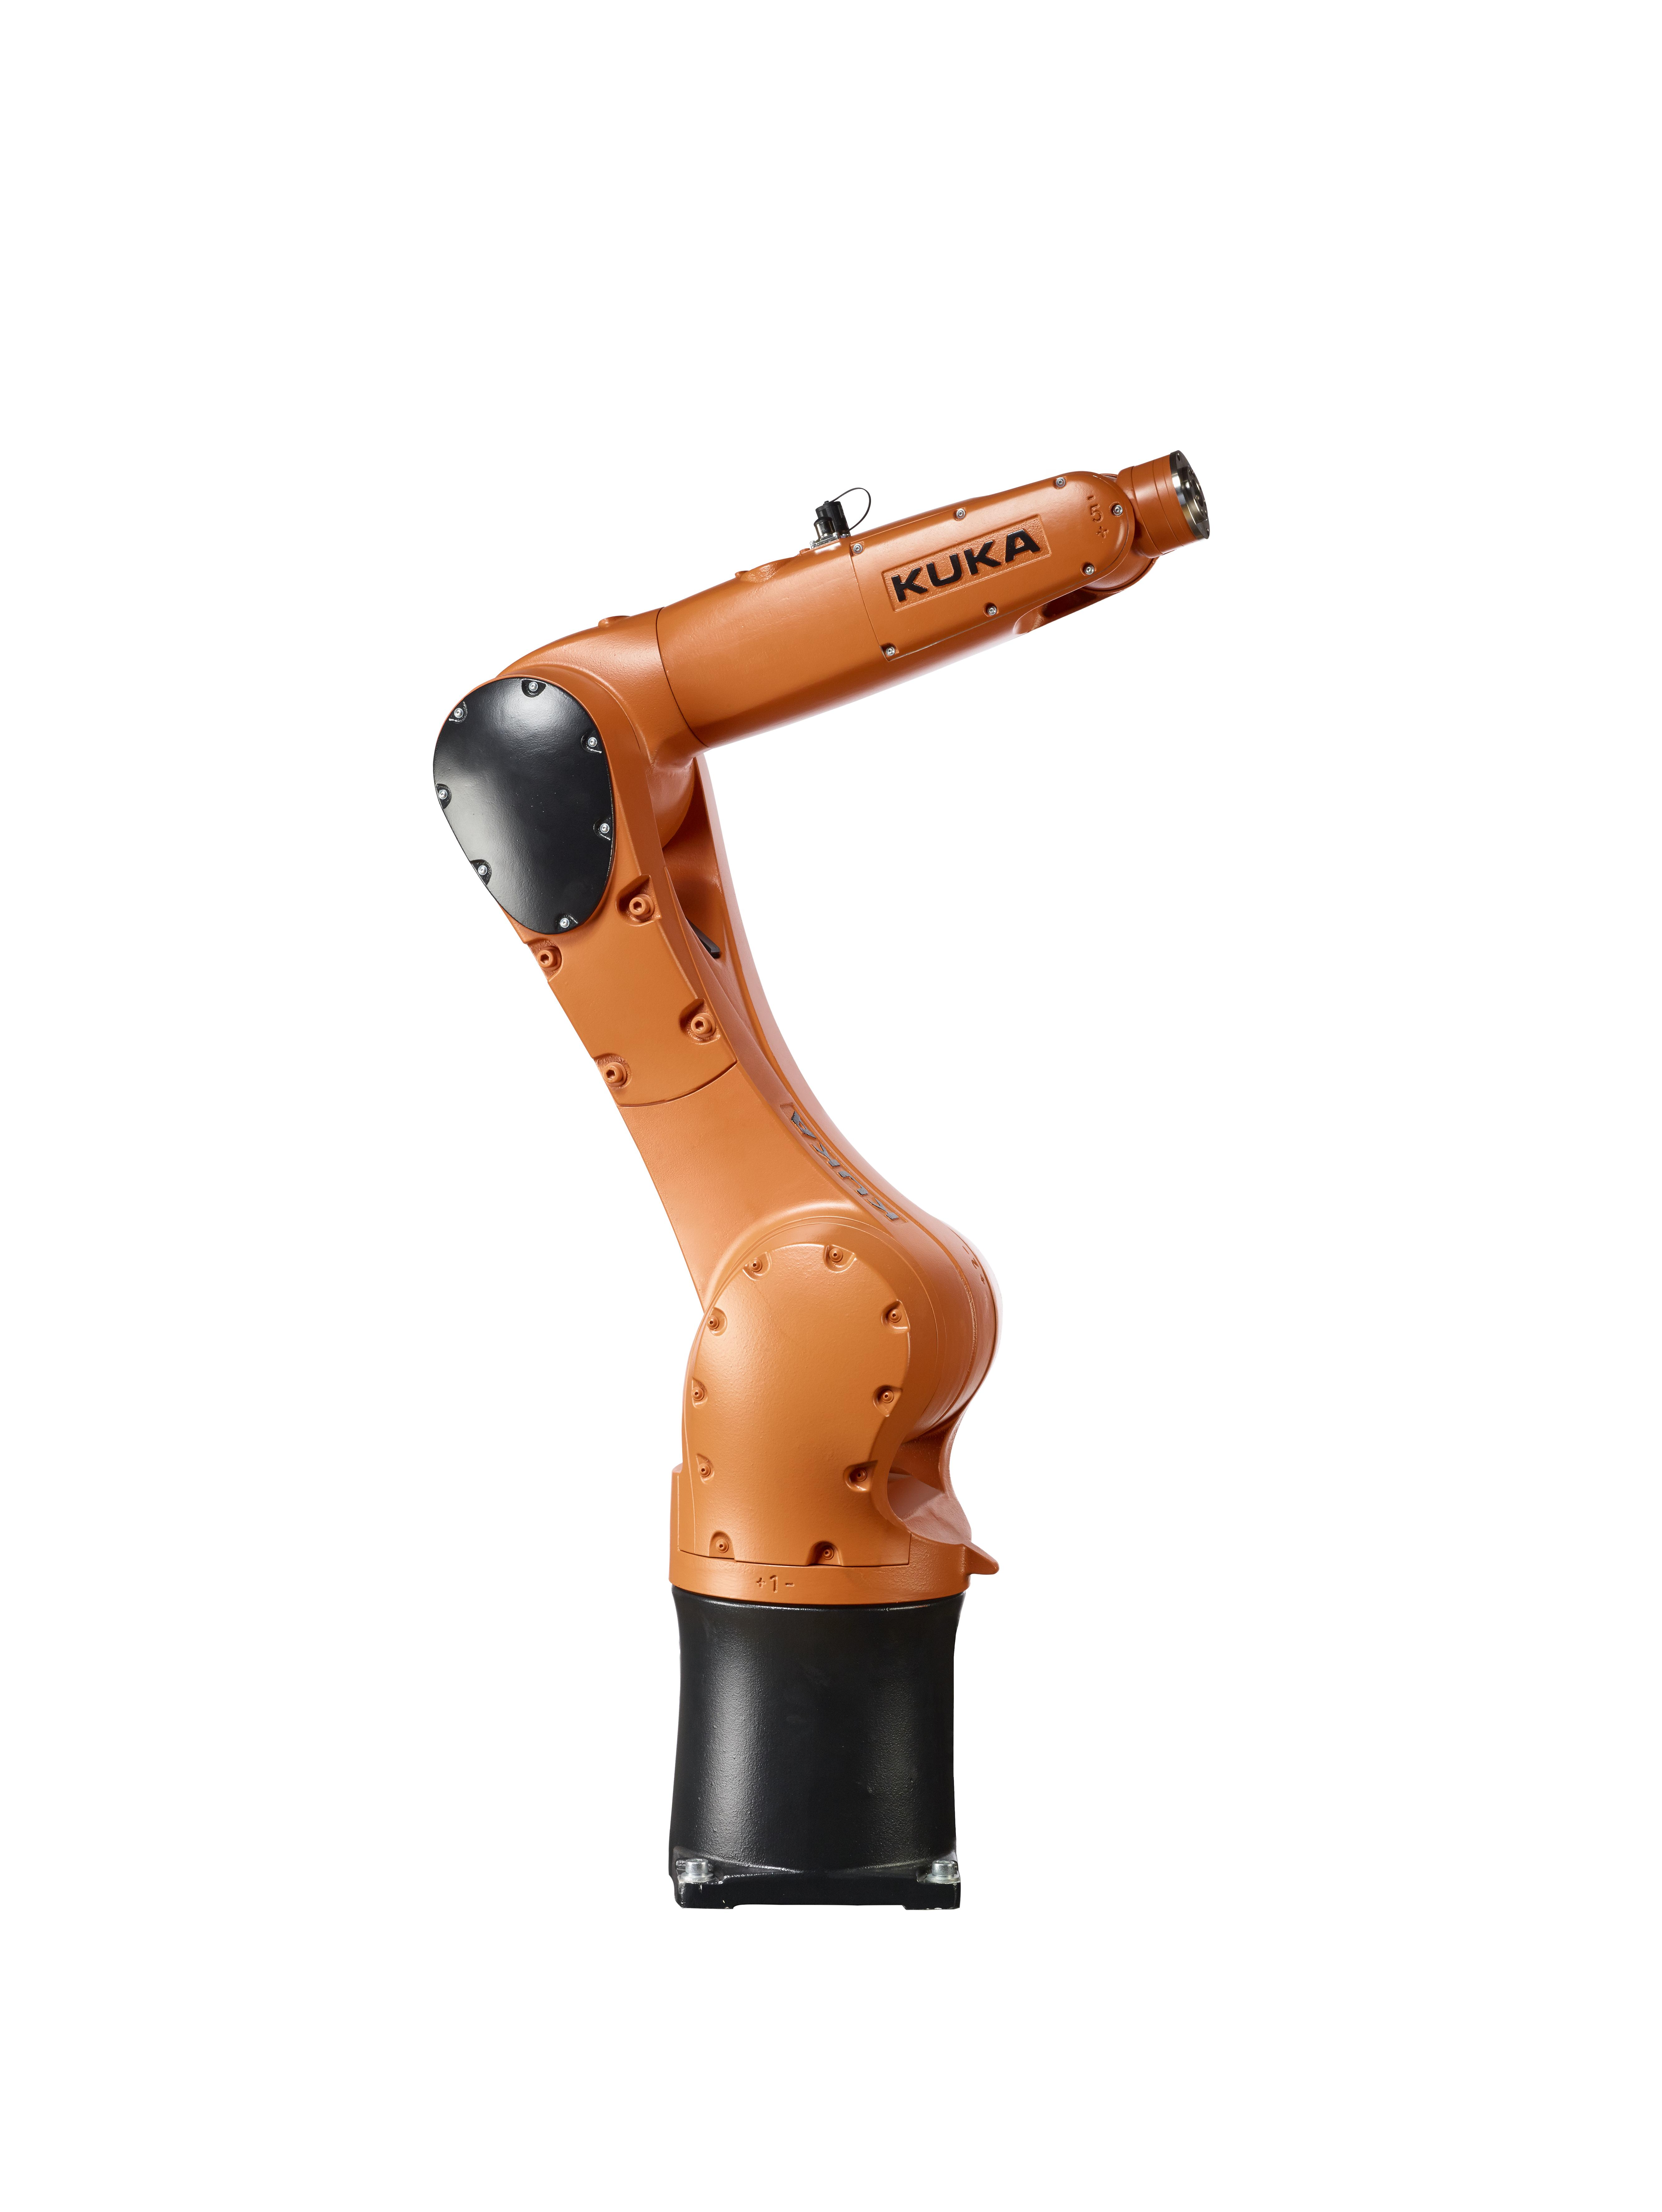
\includegraphics[width=0.5\textwidth]{Images/Task2/KUKA_KR6_R900_sixx_(Agilus).jpeg}
    \caption[KUKA KR6 R900 sixx (Agilus) robot]{The KUKA KR6 R900 sixx (Agilus) robot.}
    \label{fig:KUKA_Agilus}
    \source{\url{https://www.robot72.ru/catalog/promyshlennye-roboty/roboty-kuka/kr-6-r900-sixx/}}
\end{figure}
%source for the picutre: https://www.robot72.ru/catalog/promyshlennye-roboty/roboty-kuka/kr-6-r900-sixx/

In figure \label{fig:robot_frames} the Space $<s>$ frame and body frame $<b>$ are defined and the most important dimensions are given and enumerated. On the left figure the robot is in its x-y plane. The righthand-rule defines the z-axis out of the image towards the spectator. On both images, the robot is in the configuration 
\begin{equation}
    \theta =
    \begin{bmatrix}
    0 & −\pi/2 & \pi/2 & 0 & 0 & 0
    \end{bmatrix}
    ^{T}
\end{equation}
\begin{figure}[H]
    \centering
    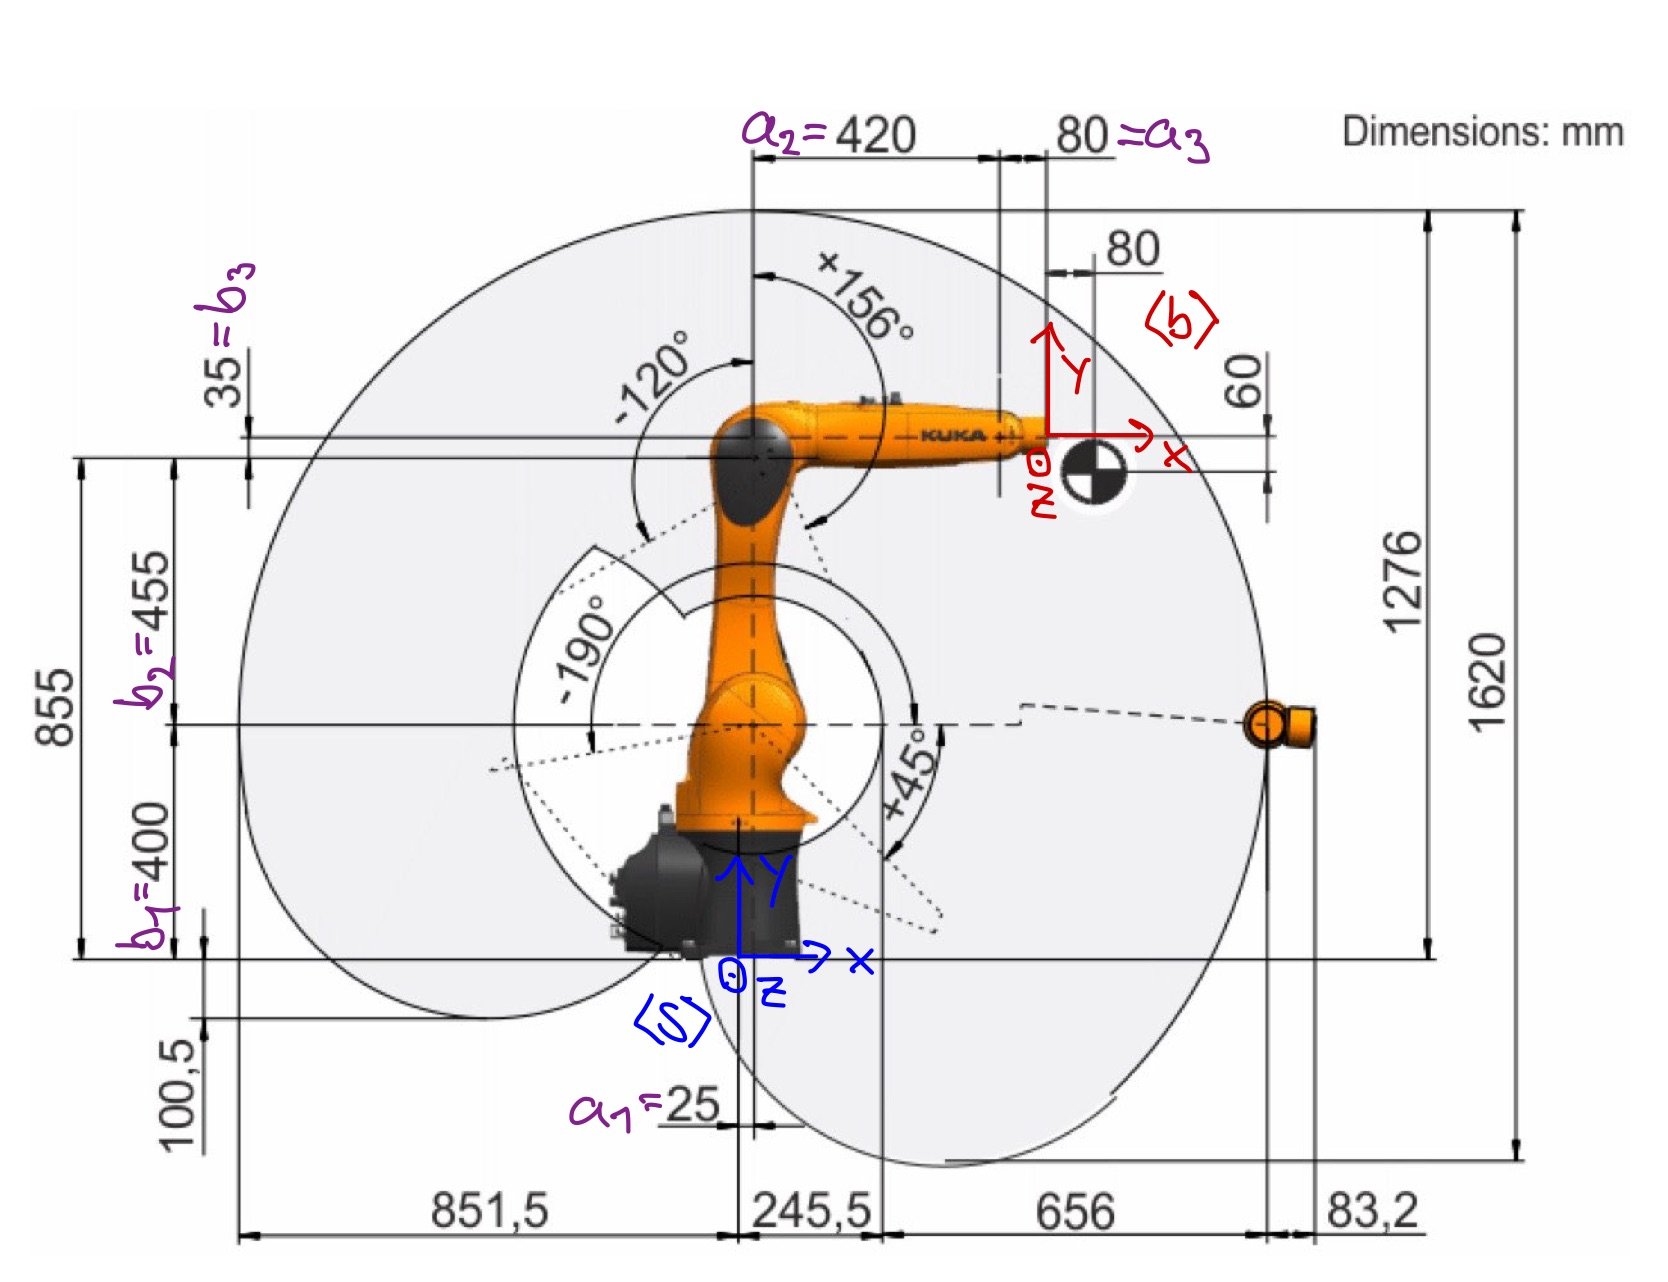
\includegraphics[width=0.6\textwidth]{Images/Task2/robot_dimensions2.jpg}
    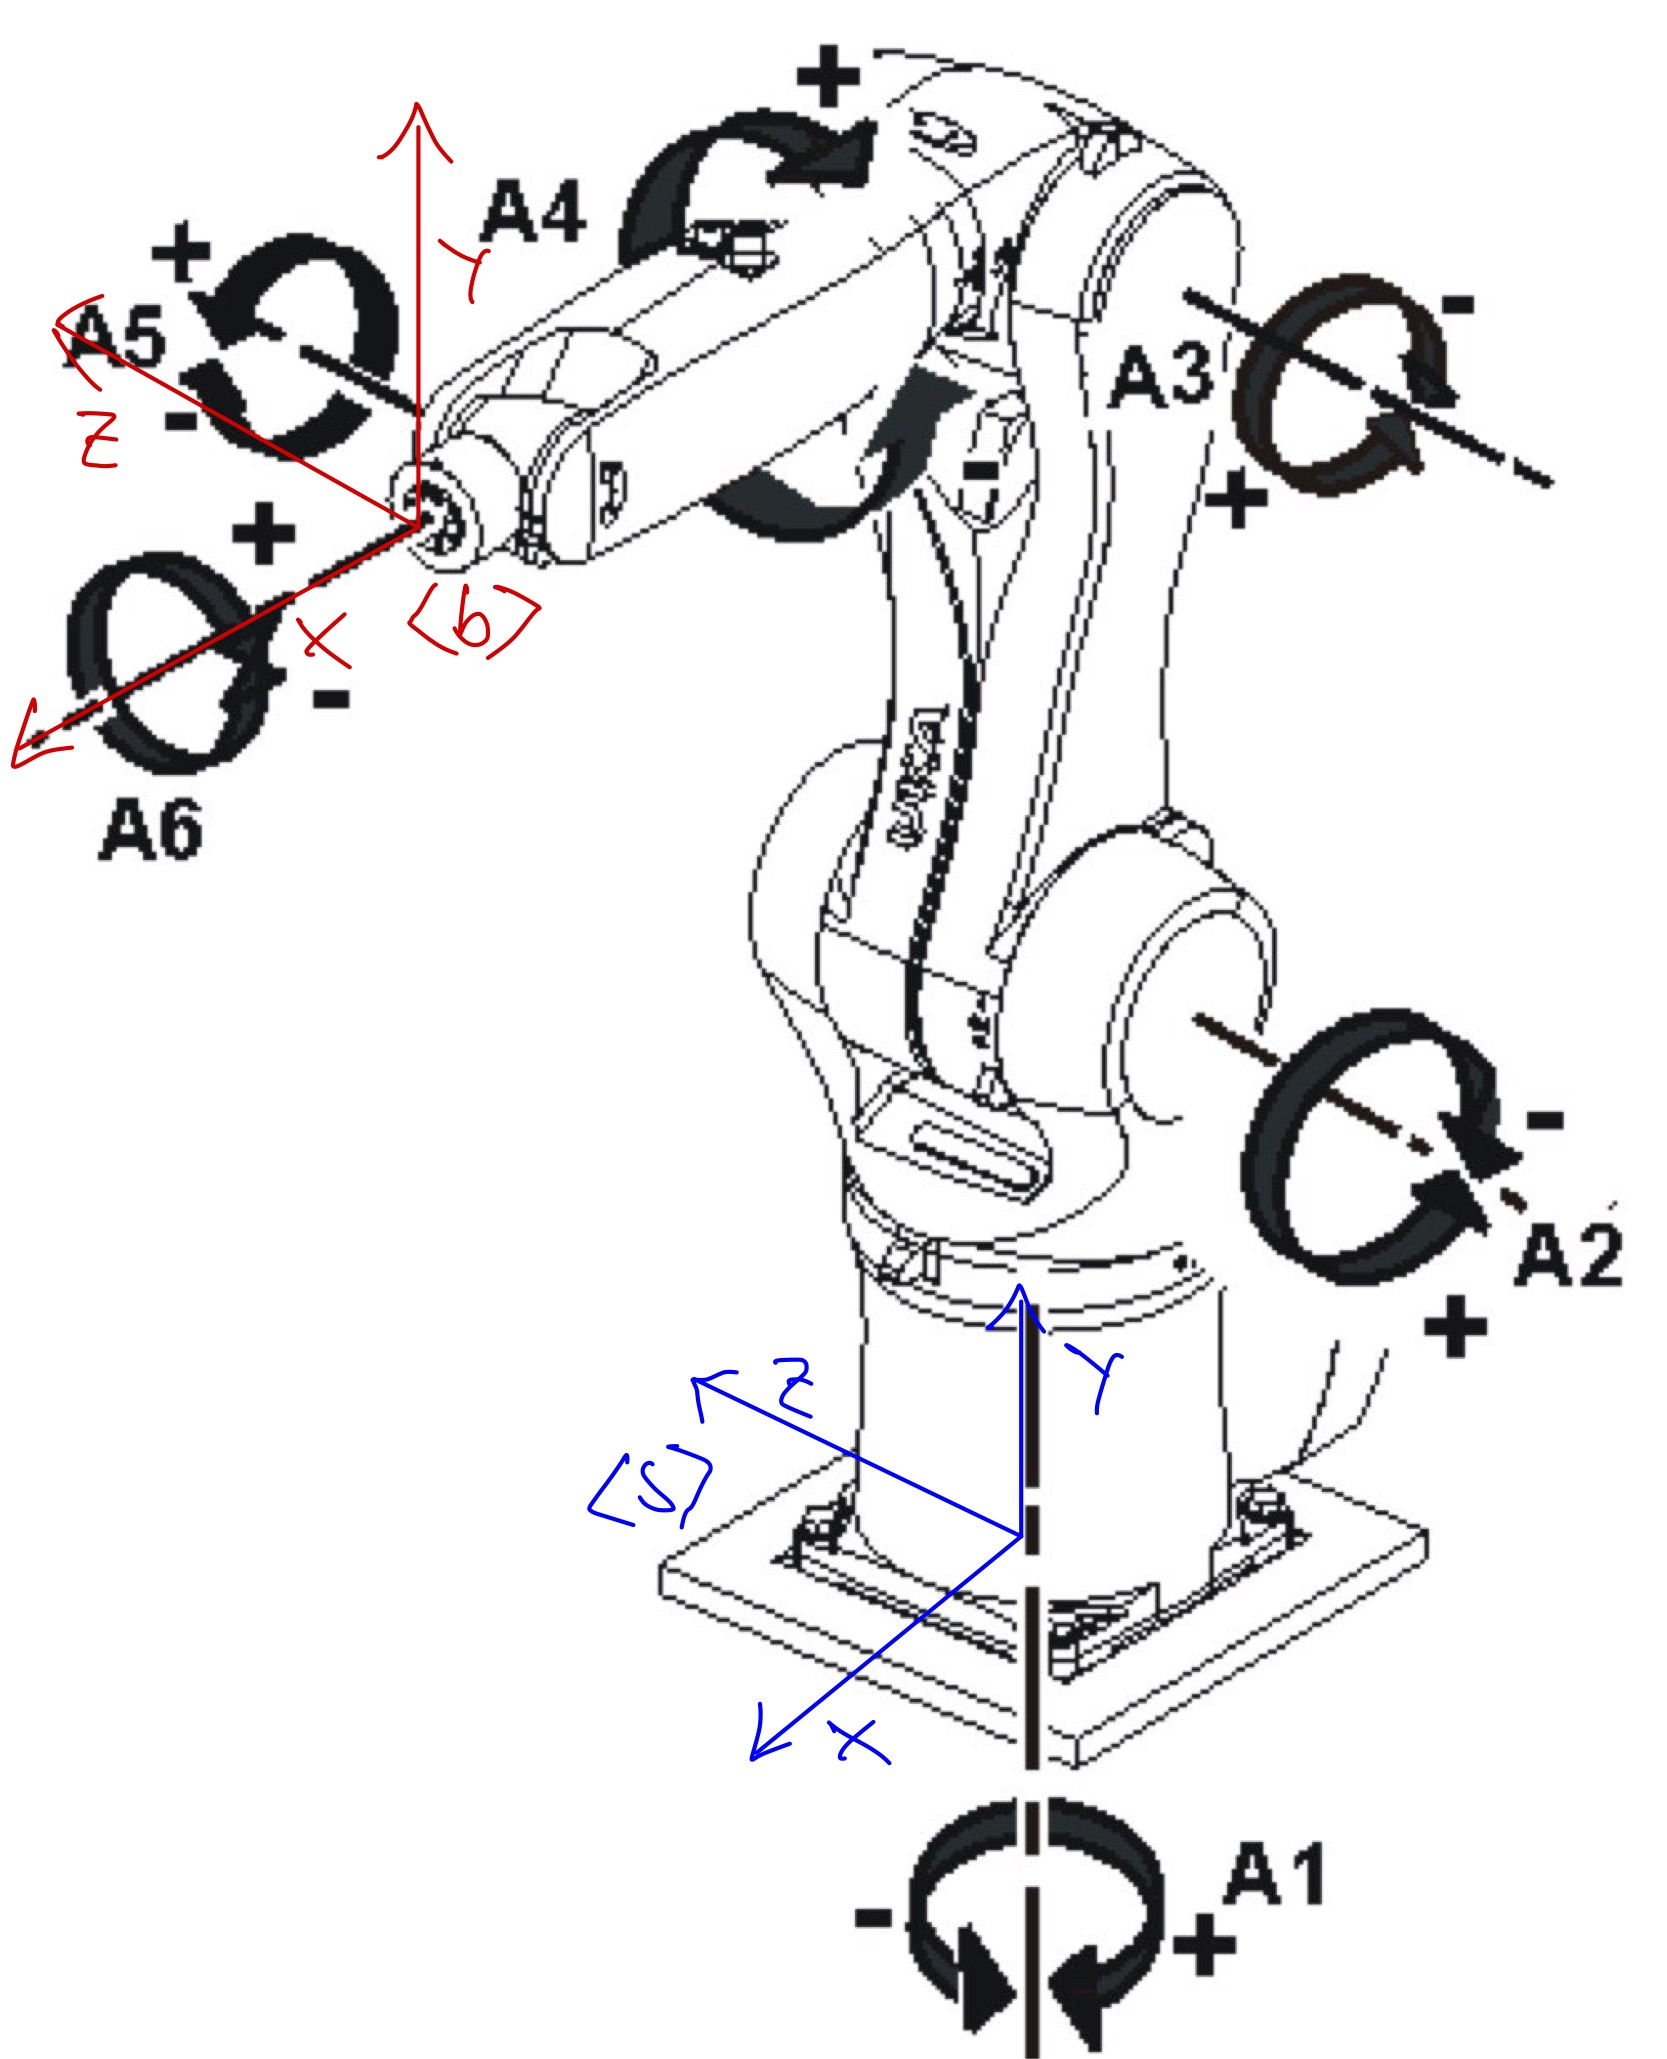
\includegraphics[width=0.3\textwidth]{Images/Task2/robot_axis2.jpg}
    \caption[Frames of the robot]{Space $<s>$ frame (blue) and body frame $<b>$ (red) and the most important dimensions (violet) to the left. Axis and rotational direction on the right.}
    \label{fig:robot_frames}
    \source{Projecttext}
\end{figure}

\subsection{Task2.1 DH of Agilus robot}
\subsubsection{Relationship}

\subsection{Task 2.2 End-effector zero position configuration}
%insert a picture of the robot in his 0 position.
While in in figure \ref{fig:robot_frames} the robot is not is its zero position, he is figure X. Since both $<s>$ $<b>$ frames are in the same plane and in the same direction, the The configuration is end-effector zero position configuration is quite easy to deduce by inspection. The matrix is given by
\begin{equation}
    M = 
    \begin{bmatrix}
    1 & 0 & 0 & a1+b2+a2+a3 \\
    0 & 1 & 0 & b1+b3 \\
    0 & 0 & 1 & 0 \\
    0 & 0 & 0 & 1
    \end{bmatrix}
\end{equation}

\subsubsection{Task 2.3 Space frame screw axis}
To determine the space frame screw axes $Si$ for the Agilus robot.

\begin{figure}[H]
    \centering
    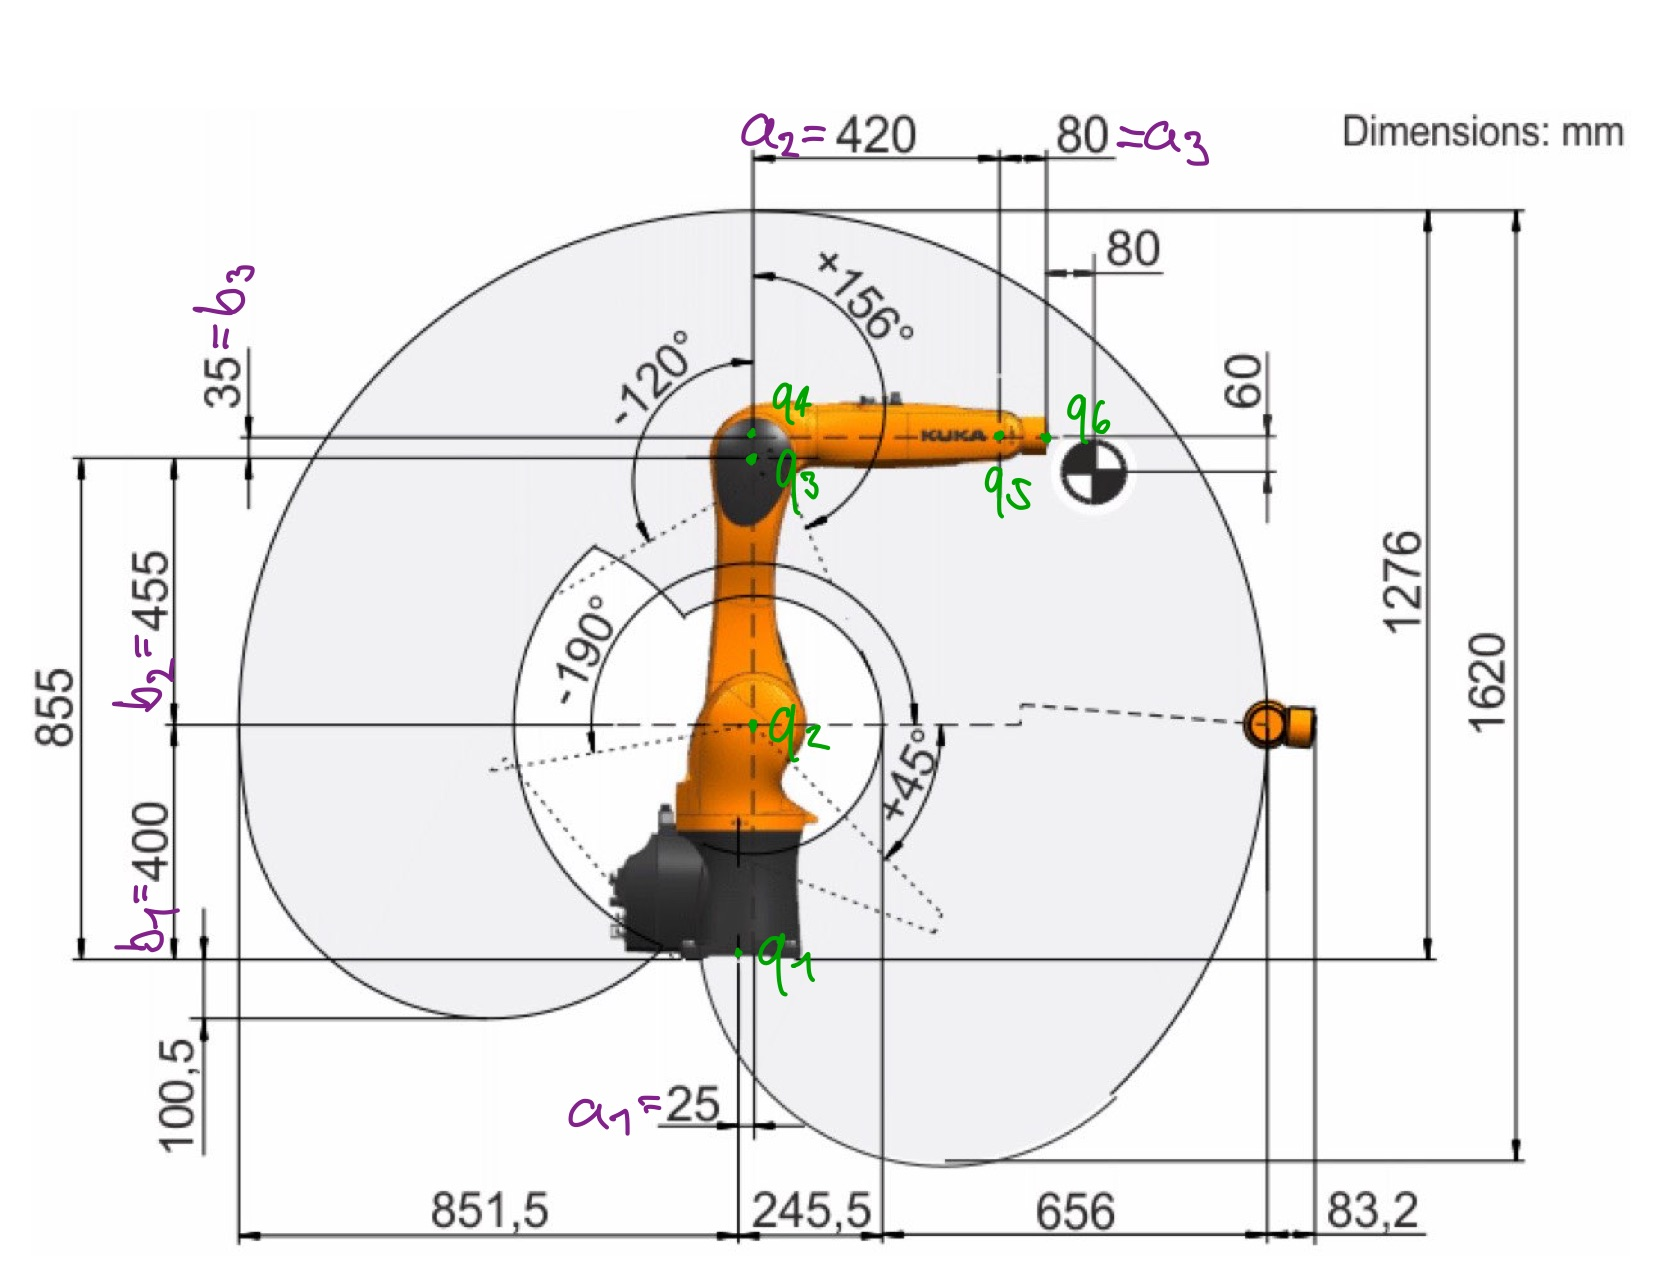
\includegraphics[width=0.6\textwidth]{Images/Task2/robot_q.jpg}
    \caption[q-positions]{The postion of q for each axis is shown.}
    \label{fig:robot_q}
    \source{Projecttext}
\end{figure}

\begin{table}[]
\begin{tabular}{|l|l|l|l|}
\hline
$i$ & $\omega$ & $q$ & $v$ \\ \hline
1 & $(0, -1, 0)$ & $(0, 0, 0)$ & $(0, 0, 0)$ \\ \hline
2 & $(0, 0,-1)$ & $(a1,b1,0)$ & $(-b1, a1, 0)$ \\ \hline
3 & $(0, 0,-1)$ & $(a1,b1+b2,0)$ &  \\ \hline
4 & $(-1, 0, 0)$ & $(a1,b1+b2+b3,0)$ &  \\ \hline
5 & $(0, 0,-1)$ & $(a1+a2,b1+b2+b3,0)$ &  \\ \hline
6 & $(-1, 0, 0)$ & $(a1+a2+a3,b1+b2+b3,0)$ &  \\ \hline
\end{tabular}
\caption{$\omega_i$, $q_i$ and $v_i$ of the screw axis in the space frame.}
\label{tab:screw-axis}
\end{table}

\subsubsection{Task 2.4 Body frame screw axis} 
%should i use numbers or variables?



